\section{Methods}

\subsection{Overview}

Our hypothesis is that performing test time adaptation on cell segmentation will improve cell tracking performance since the associations are based on simple metrics such as IoU and Euclidean distance of the centroids~\cite{bragantini2024ultrack}. In our approach, we assume to have a pre-trained network available that was trained on a source dataset. Since Cellpose~\cite{stringer2021cellpose} is still one of the state-of-the-art algorithms for the task of cell instance segmentation, we choose that to be our baseline algorithm and build TTA framework on top of that. In the following sections, we will discuss preliminaries on Cellpose~\cite{stringer2021cellpose}, TTA, and our proposed framework. 



\subsection{Cell Segmentation}

To test our hypothesis, we use one of the state-of-the-art cell instance segmentation algorithms as our segmentation framework Cellpose~\cite{stringer2021cellpose}. It is pretrained on diverse datasets and has good generalization capability. However, it is not pretrained on all imaging modalities or cell types, rendering it less useful in out-of-distribution datasets. We propose to utilize their pretrained model and perform test-time adaptation. 

Here, we describe the inner workings of Cellpose~\cite{stringer2021cellpose}: given an image $I$, the model uses a network $f$ to produce a dense, pixel-wise feature $\bm{Z} = f(I)$, where $ \bm{Z} = [Z_1, Z_2, Z_3] \in \mathbb{R}^{h \times w \times 3}$. Given the feature $\mathbf{z} = [z_1, z_2, z_3] \in \bm{Z}$ for some pixel $i$, then $\bm{z} \doteq (z_1, z_2)$ has the meaning of gradient pointing towards the center of the cell structure to which pixel $i$ belongs. Collectively, $(Z_1,Z_2)$ form a \emph{gradient flow}. Instead, $z \doteq z_3$ represents the unnormalized score indicating the probability of pixel $i$ to belong to a cell structure. Note that with this notation, the feature $\mathbf{z}$ can be written as $\mathbf{z} = [\bm{z}, z]$. The network $f$ is trained in a supervised manner with pixel-wise instance segmentation loss
\begin{equation}
  \mathcal{L}_i^{IS} = (z_1 - \mathtt{g_x})^2 + (z_2 - \mathtt{g_y})^2 + \nu H(\mathtt{m},\sigma(z))  \; ,
\end{equation}
where, for pixel $i$,  $(\mathtt{g_x}, \mathtt{g_y})$ represents the ground-truth gradient label with unit $\ell_2$-norm, $\mathtt{m} \in \{0, 1\}$ is the binary mask label indicating absence/presence of a cell structure, $\sigma(z) \doteq 1/(1+\exp(-z))$, $H$ represents the binary cross-entropy, and $\nu$ is a hyperparameter set to $0.04$. The pixel-wise loss contributions are then aggregated into a final loss $\mathcal{L}^{IS} = \sum \mathcal{L}_i^{IS}$ for the image $I$.


Given the feature $\bm{Z}$, the cell instance segmentation head $g$ produces the mask $Y = g(\bm{Z})$, where for pixel $i$, the predicted label $y$ is a number in the set $\{0, 1, \cdots, N \}$, with $N$ being the total number of cell instances segmented. Pixels belonging to the same cell instance have same label, and $y=0$ indicates absence of a cell instance. 


<<<<<<< HEAD
\subsection{Test-Time Adaptation Model}

At test-time, we follow two TTA constraints: (i) no source data available and (ii) no target labels available. In this setting, we want to perform the adaptation in a fully unsupervised manner. Once we have a pre-trained Cellpose~\cite{stringer2021cellpose} model available, we will utilize its predictions on the target data to perform the adaptation. Here,   

\subsubsection{Self-Entropy}
=======
\subsection{Test-Time Adaptation Loss Computation}

At test-time, we follow two TTA constraints: (i) no source data available and (ii) no target labels available. In this setting, we want to perform the adaptation in a fully unsupervised manner. Once we have a pre-trained Cellpose~\cite{stringer2021cellpose} model available, we will utilize its predictions on the target data to perform the adaptation. Here,   

\subsubsection{Self-Entropy}\label{sec:tta-se}
>>>>>>> origin/master
One of our first objectives is to calculate the Shannon entropy~\cite{shannon1948mathematical} of the mask probability predictions. Shannon entropy~\cite{shannon1948mathematical} allows us to quantify the model uncertainty in the model predictions. As it refers to the uncertainty of the model, we could also utilize this information as a metric to decide which predictions are confident predictions. It is especially crucial as data distributions can change during inference. As our mask predictions are given by $\sigma(z)$, our Shannon entropy~\cite{shannon1948mathematical} becomes the following:

\begin{equation}
    \mathcal{L}_i^{SE} = -\sigma(z) \log \sigma(z) \; ,
\end{equation}

However, since our mask predictions refer to a binary crossentropy task and do not possess a probability distribution over $k$ classes, we redefine the entropy as the following:
\begin{equation}
    \mathcal{L}_i^{SE} = -(\sigma(z) \log \sigma(z) + (1-\sigma(z)) \log (1-\sigma(z))) \; ,
\end{equation}

Now that we calculated $\mathcal{L}^{SE}$ for the binary mask predictions, we can use this information to collect more confident prediction. We choose a threshold $\delta$ that describes if the $\mathcal{L}_i^{SE}$ is lower than the threshold, then the predictions are confident enough. It is given by $\hat{\bm{z}} = \bm{z}[\mathcal{L}^{SE}<\delta]$. Further, once the indices are collected, we choose a probability threshold $p$ that determines if the original predictions have large enough probability to be considered a valid prediction which is given by $\hat{\bm{z}} = \hat{\bm{z}}[\sigma(z)<p]$. Now, we have a refined set of indices which will be useful in the next section. 

<<<<<<< HEAD
\subsubsection{Contrastive Flow Loss}
Proposed framework employs a contrastive prediction task for enhancing gradient flow features of the target pixels. \cite{keaton2023celltranspose} first proposed to utilize a contrastive objective in gradient flow alignment task; however, their framework is supervised whereas our framework performs contrastive learning in a self-supervise manner. We decide a positive sample with refined binary mask from  $\hat{z}$ with predictions $\mathbb{I}[\hat{z}>p]$, that is $\hat{z_+}=\hat{z}=1$. We further decide the gradient flow features $\hat{\bm{z}}_+$ closest to a prediction  $\hat{\bm{z}} = (z_1,z_2)$ according to a similarity metric. In our case we use cosine similarity given by $s(\bm{u},\bm{v})\doteq\frac{\bm{u}^T\bm{v}}{\| \bm{u} \| \| \bm{v}\| }$, where $\| \cdot \|$ denotes $l_2$-norm.  
=======
\subsubsection{Contrastive Flow Loss} \label{sec:tta-cfl}
Proposed framework employs a contrastive prediction task for enhancing gradient flow features of the target pixels. \cite{keaton2023celltranspose} first proposed to utilize a contrastive objective in gradient flow alignment task and we follow their formulation in this paper; however, their framework is supervised whereas our framework performs contrastive learning in a self-supervise manner. We decide a positive sample with refined binary mask from  $\hat{z}$ with predictions $\mathbb{I}[\hat{z}>p]$, that is $\hat{z_+},\hat{z}>p$. We further decide the gradient flow features $\hat{\bm{z}}_+$ closest to a prediction  $\hat{\bm{z}} = (z_1,z_2)$ according to a similarity metric. In our case we use cosine similarity given by $s(\bm{u},\bm{v})\doteq\frac{\bm{u}^T\bm{v}}{\| \bm{u} \| \| \bm{v}\| }$, where $\| \cdot \|$ denotes $l_2$-norm.  We collect the set of negative samples $\mathcal{N}_i = \{ \hat{\bm{ z}}_- \; | \; s(\hat{\bm{ z}}_+,\hat{\bm{ z}}_-) < \theta, \hat{z}_- > p\}$, where $\theta$ is an appropriate hyperparameter threshold we choose. Once the positive and negative samples are collected, we deploy our contrastive objective for pixel $i$ that will attempt to pull the positive pairs $(\hat{\bm{z}}, \hat{\bm{z}_+})$, at the same time pushing away the negative pairs $(\hat{\bm{z}}, \hat{\bm{z}}_-)$.  \cite{wang2021understanding} suggests clever hard-mining strategies for learning with a contrastive objective in which the hard-mining of negative samples limits the need for a huge number of negative samples at the same time improving the convergence speed. Since our objective is adapting at test time, fast convergence will benefit the algorithm grately. Therefore, in our case, similar to \cite{keaton2023celltranspose}, we follow hard-mining sampling strategy for negative samples. In essence, $\mathcal{N}_i$ is composed of a set if pixels that are close to the positive samples. Please refer to  \cite{keaton2023celltranspose} for the details. \\

Given a batch of target image patches, each patch is paired with another patch from the same batch. We then compute the contrastive flow loss aggregating all the components coming from the all the valid pixels, i.e.,  $\hat{z}_- > p$. 
Now the loss function becomes the following:
>>>>>>> origin/master

\begin{equation}
    \small
    \mathcal{L}_i^{CF} = - \log \frac{\exp( s (\hat{\bm{ z}}, \hat{\bm{ z}}_+)/\tau )}{ \exp( s (\hat{\bm{ z}}, \hat{\bm{ z}}_+)/\tau ) + \sum_{\hat{\bm{ z}}_- \in \mathcal{N}_i} \exp( s (\hat{\bm{ z}}, \hat{\bm{ z}}_-)/\tau ) }\\
    \label{eq-contrastive-flow-loss}
  \end{equation}
where $\tau$ refers to a temperature parameter we choose. 

<<<<<<< HEAD
% \begin{figure}[t]
%     \centering
%     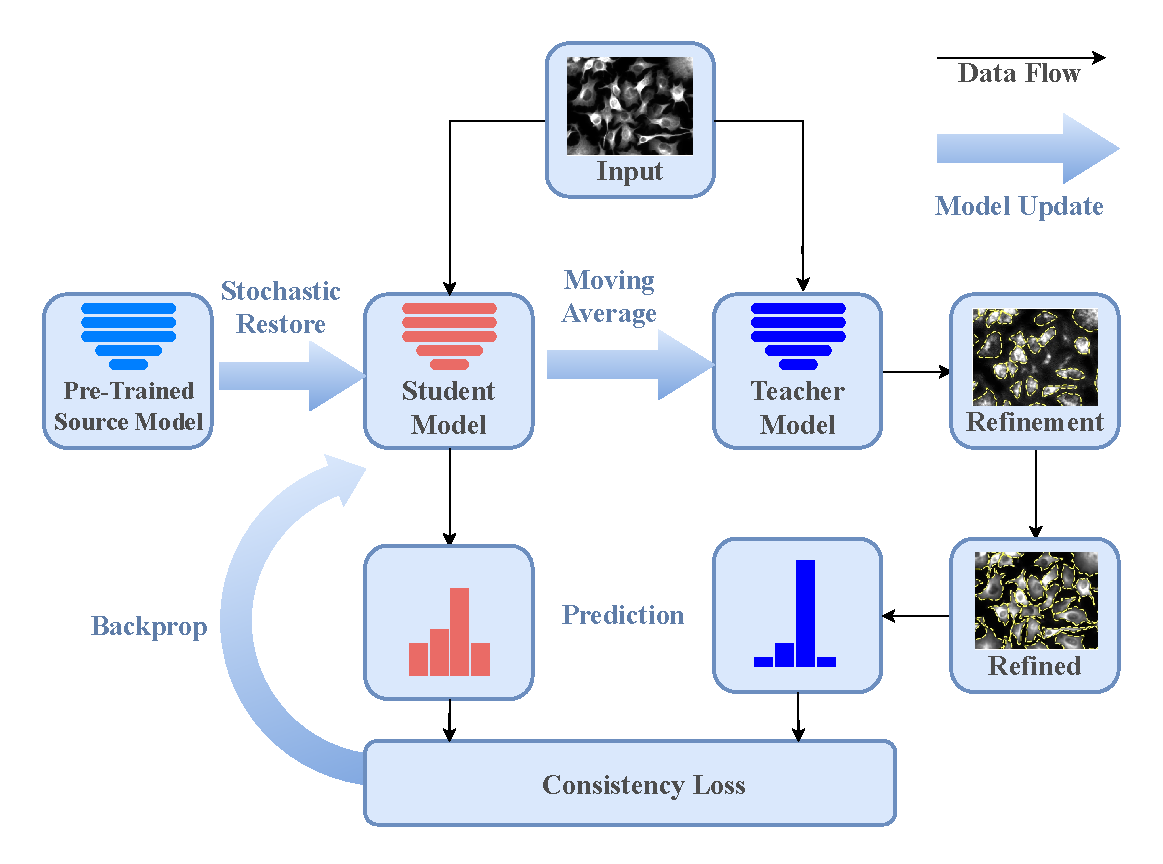
\includegraphics[width=9cm]{figs/project_proposal.pdf}
%     \caption{Overall Framework.}
%     \label{fig:overall_framework}
% \end{figure}

% \subsection{Training Gaussian Splats Algorithm}

% Radiance fields are a new form of 3d representation which relies on novel differentiable ray-marching, in this talk we will discuss two types Neural Radiance Fields (NeRF) and Gaussian Splatting (GS).   In brief, a radiance field is a learnable representation of a scene, in the case of the NeRFS a large MLP is used as the mechanism and in GS a variable list of ellipsoids.  A raycast is a form of graphics rendering in which the emission of photons onto a pixel is calculated by tracking the reflection of light.  For instance, to find the color of the middle pixel of an image, a ray can be calculated in the opposite direction of how light is received by the camera.  Usually in the case of raycast, for simplicity, once the ray hits an object in the 3d scene it stops and the color of the hit object is blended into that pixel.  \\

% Instead of the ray cast ending after an arbitrary number of reflections, the rays’ direction is not affected by reflection.  Each perceptron in NeRF or Ellipsoid in GS is associated with an emission of light which adds its contribution to the ray by integrating the contribution of each perceptron or ellipsoid to the ray small changes to the light emitted are captured by the alpha-blending equation. Each of these are trained by taking training samples and finding the divergence between the rendering at the current training step compared to the known ground truth image.  In order, to have this information though you need to also know the pose of the camera relative to the scene during training which can be a major impediment to applying a radiance field method. In this case we have the benefit of a closed system where we can define the position of the viewer based on the geometry of the original imaging system which is published information.  \\  

% \subsubsection{Dynamic Gaussian Splatting}
% \label{sec:related_works_gaussian_splatting}
% Importantly for this investigation we must go beyond the original scope of Gaussian splatting to accommodate the time-dynamic nature of the data to apply it to tracking.

% In our case, we are going to combine the techniques of \cite{Zhou2023-zg} and \cite{Bae2024-xu}. In \cite{Zhou2023-zg}, they demonstrate the ability to optimize a Gaussian field that can approximate both the images and the features from a novel view. In order to take into account the time-dynamics, we have to integrate the ideas of \cite{Bae2024-xu}. In order to deal with dynamic the field is seperated into static components and dynamic deformations.  The static components are those that are well-modelled by the initial GAN. The deformations are further divided into "slow" and "fast" changes so that the slow changes can be handled by a coarse model followed by a fine deformation model to implement the fast changes.  The potential downside of \cite{Bae2024-xu}, is that it requires optimization on a per-gaussian basis so it is sensitive to complexity in the scene, but in our domain we have a situation where the objects of interest can be represented with very few gaussians without effecting the appearance based losses.

% \subsection{Refinement}
% The refinement module processes three inputs to construct a more refined mask. These three inputs are: the raw image volume, initial segmentation produced by the Cellpose~\cite{stringer2021cellpose} base model, and Gaussian splats constructed from the raw image volume. On the architecture side, this module shares the exact same architecture as CellpoSe~\cite{stringer2021cellpose}, except the number of input channels. Please refer to ~\Cref{fig:refinement}.

% \begin{figure}[t]
%     \centering
%     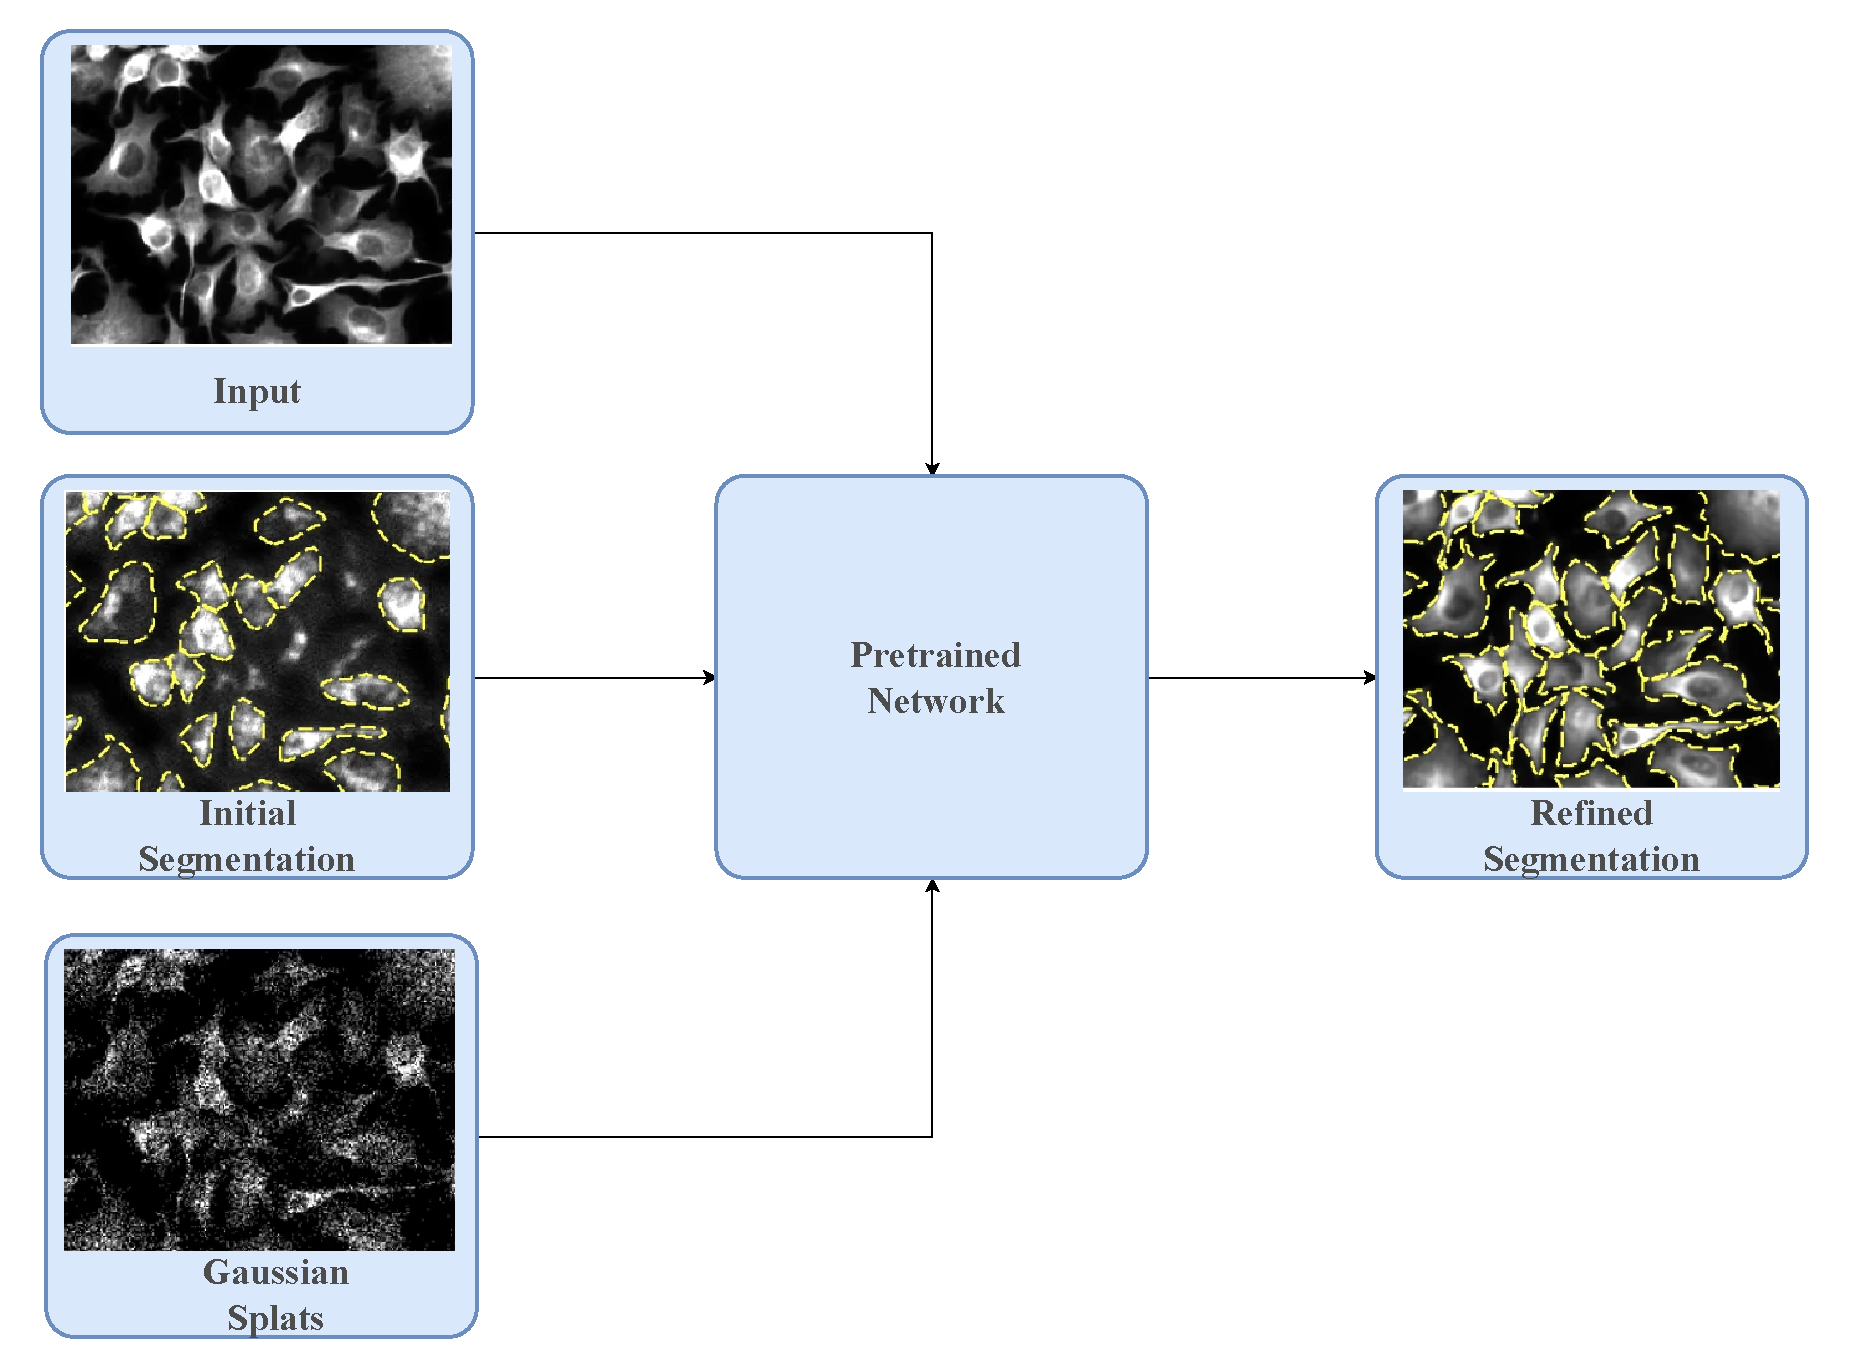
\includegraphics[width=9cm]{figs/refinement.pdf}
%     \caption{Refinement Strategy.}
%     \label{fig:refinement}
% \end{figure}
=======
\subsubsection{Adaptation Loss}
In \cref{sec:tta-se}, we calculate self-entropy for the binary mask predictions and in \Cref{sec:tta-cfl}, we calculate a contrastive object to enhance the gradient flow estimations. We combine this two losses for the model update at test time as shown below:
\begin{equation}
    \small
    \mathcal{L}^{TTA} = \lambda_1\frac{1}{| \mathcal{M}_1 |} \sum_{\mathcal{M}_{1}} \mathcal{L}^{SE}_i + \lambda_2\frac{1}{| \mathcal{M}_2 |} \sum_{\mathcal{M}_2} \mathcal{L}^{CF}_i \; .
    \label{eq-tta-loss}
  \end{equation}
Where, total pixel belonging to the target patch, we define it by $\mathcal{M}_1$, and the valid pixels we define that set by $\mathcal{M}_2$. $\lambda_1$ and $\lambda_2$ are the weight parameters for the loss. This combination of losses is used to perform the adaptation. In the next section, we will discuss what parameters we want to update during TTA. 

\subsection{Test-Time Adaptation Parameter Updates}
>>>>>>> origin/master
